\chapter{张量融合范畴与弦网模型}

\section{范畴论基础}

\emph{范畴论} (category theory)\cite{baez2011physics,maclane2013categories,beer2018categories} 用以抽象地刻画一些数学结构之间的关系,它主要描述了“对象”之间的作用,即\emph{映射} (mapping)。拓扑序理论中所研究的,正是带有了某些附加结构的范畴。

一个\emph{范畴} $\mathcal{C}$ 由其中的\emph{对象} (object) $x\in\mathcal{C}$ 和这些对象之间的\emph{态射} (morphism) $f\colon x\to y$ 组成。对象之间的态射满足以下三个条件:
\begin{itemize}
  \item \emph{复合性} (composition):对于范畴 $\mathcal{C}$ 中的对象 $x$、$y$、$z$,若 $f\colon x\to y$ 和 $g\colon y\to z$ 为态射,则存在复合态射 $g\circ f\colon x\to z$;
  \item \emph{结合律} (associativity):若 $\mathcal{C}$ 中有态射 $f\colon x\to y$、$g\colon y\to z$、$h\colon z\to w$,则有
    \begin{equation}
      (h\circ g)\circ f = h\circ (g\circ f);
    \end{equation}
  \item \emph{单位元} (identity):对于 $\forall x\in\mathcal{C}$,都存在恒等态射 $\id_x\colon x\to x$,使得
    \begin{equation}
      f \circ \id_x = \id_x \circ f = f, \quad \forall f\colon x\to y.
    \end{equation}
\end{itemize}
态射也可记为 $f\in\Hom_{\mathcal{C}}(x,y)$,其中 $\Hom_{\mathcal{C}}(x,y)$ 称为同态集 (hom-set)。如果 $x=y$,则称 $f$ 为\emph{自同态} (endomorphism),记为 $f\in\End_{\mathcal{C}}(x)$。

\emph{函子} (functor) 是范畴之间保结构的映射。具体而言,对于范畴 $\mathcal{C}$、$\mathcal{D}$,函子 $F\colon\mathcal{C}\to\mathcal{D}$ 会将 $\mathcal{C}$ 中的对象 $x$ 映射到 $\mathcal{D}$ 中的对象 $F(x)$,而将 $\mathcal{C}$ 中的态射 $f\colon x\to y$ 映射到 $\mathcal{D}$ 中的态射 $F_f\colon F(x)\to F(y)$,并且保持复合性与单位元的成立,即
\begin{align}
  F_{\id_x} &= \id_{F(x)} \colon F(x) \to F(x), \quad \forall x\in\mathcal{C}, \\
  F_{g\circ f} &= F_g \circ F_f \colon F(x) \to F(z), \quad \forall f\colon x\to y, \, g\colon y\to z.
\end{align}

在函子之上可进一步定义\emph{自然变换} (natural transformation)。对于两个函子 $F\colon\mathcal{C}\to\mathcal{D}$ 和 $G\colon\mathcal{C}\to\mathcal{D}$,自然变换 $\tau\colon F\Rightarrow G$ 由其分量 $\tau_x$(这是范畴 $\mathcal{D}$ 中的一个态射)定义:
\begin{equation}
  \tau_x\colon F(x)\to G(x), \quad \forall x\in\mathcal{C},
\end{equation}
它满足
\begin{equation}
  \tau_y \circ F_f = G_f \circ \tau_x, \quad \forall f\colon x\to y.
\end{equation}
如图~\ref{fig:natural-transformation},自然变换可以用交换图来直观地表示。若 $\tau$ 的每一分量 $\tau_x$ 均可逆(即存在 $\tau_x^{-1}$ 使得 $\tau^{-1}_x\circ\tau_x=\id_{F(x)}$ 且 $\tau_x\circ\tau^{-1}_x = \id_{G(x)}$),则称其为\emph{自然同构} (natural isomorphism),我们用 $\similarrightarrow$ 来表示。

\begin{figure}[htb]
  \centering
  \begin{tabular}{c@{\qquad}c}
    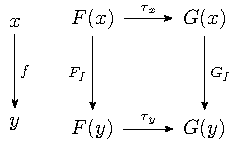
\includegraphics{images/natural-transformation-1.pdf} &
    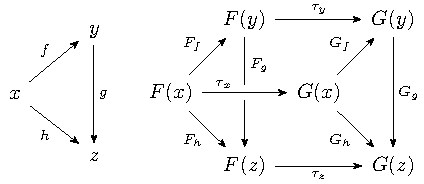
\includegraphics{images/natural-transformation-2.pdf} \\
    (a) & (b)
  \end{tabular}
  \caption[自然变换对应的交换图]{自然变换对应的交换图。(a) 此图是“可交换的”,即从 $F(x)$ 到 $G(y)$ 的两条路径等价;(b) 对于结合律的“提升”,图中三棱柱的三个侧面都是可交换的。}
  \label{fig:natural-transformation}
\end{figure}

\begin{example}
  对于任意的交换环 $K$,以其中元素构成的 $n\times n$ 的非奇异矩阵组成了一般线性群 $GL_n(K)$。对于环同态 $f\colon K\to L$,显然可以构建群同态 $GL_n f\colon GL_n(K)\to GL_n(L)$。因此,$GL_n$ 即为交换环范畴 $\mathbf{CRng}$ 到群范畴 $\mathbf{Grp}$ 的函子。

  设非奇异矩阵 $M\in GL_n(K)$,则其行列式 $\det_K(M)$ 为 $K$ 中的可逆元(即单位),因而 $\det_K$ 是群同态 $GL_n(K)\to K^\times$,其中 $K^\times$ 为 $K$ 的可逆元群。另一方面,当把环同态 $f$ 限制在可逆元群上时,可得群同态 $f^\times\colon K^\times\to L^\times$,因而 $(\cdot)^\times$ 同样也是 $\mathbf{CRng}$ 到 $\mathbf{Grp}$ 的函子。根据定义,$\det\colon GL_n\Rightarrow(\cdot)^\times$ 即为自然变换,它满足 $\det_L\circ\,GL_n f=f^\times\circ \det_K$。
\end{example}

% \begin{example}
%   在 Haskell 编程语言中,类型为范畴 $\mathbf{Hask}$ 中的对象,而纯函数为态射。函子可由类型类 (type class) 来定义,例如 \verb|List| 可以将类型 \verb|T| 构造为对应的数组 \verb|[T]|,并且通过 \verb|fmap| 将以 \verb|T| 类型为参数的纯函数转换为以 \verb|[T]| 类型为参数的纯函数。自然变换则由参数多态 (parametric polymorphism) 实现。例如,一个安全的(不引发异常)返回数组首元素的函数可按下面的方式定义:
% \begin{verbatim}
%   head :: [T] -> Maybe T
%   head []     = Nothing
%   head (x:xs) = Just x
% \end{verbatim}
%   因此 \verb|head| 函数是从 \verb|List| 到 \verb|Maybe| 的自然变换。
% \end{example}

\emph{弦图} (string diagram) 可以更直观地描述范畴的概念。其中,带箭头的直线或曲线代表对象,盒子代表态射\cite{selinger2011survey,baez2011physics}:
\begin{equation}
  f\colon x\to y \quad \coloneq \quad
  \tikzinput{morphism} \, .
\end{equation}
这样态射的复合就可以表示为连在一起的两个盒子:
\begin{equation}
  \tikzinput{composition}.
\end{equation}

\section{张量范畴与融合范畴}
\label{sec:tensor-category-fusion-category}

\subsection{张量范畴}

我们可以在范畴中引入一些结构,使其具有新的特性。引入了张量积的范畴为\emph{张量范畴} (tensor category)\cite{bakalov2001lectures,muger2008tensor,maclane2013categories,beer2018categories,kong2022invitation}。它最基本也最重要的例子是向量空间(或对应的范畴 $\mathbf{Vec}$),其中的张量积结构即为两个向量空间和相应线性变换的直积。一个张量范畴 $\mathcal{C}$ 由下面的条件定义:
\begin{itemize}
  \item \emph{张量积} (tensor product) $\otimes\colon\mathcal{C}\times\mathcal{C}\to\mathcal{C}$ 和\emph{单位对象} (unit object) $\1\in\mathcal{C}$;
  \item \emph{结合子} (associator) $\alpha$,它是一个自然同构:
    \begin{equation}
      \alpha_{x,y,z} \colon (x\otimes y)\otimes z \similarrightarrow x\otimes(y\otimes z), \quad \forall x,y,z \in \mathcal{C};
    \end{equation}
  \item \emph{左右单位子} (left/right unitor),同样也是自然同构:
    \begin{equation}
      \lambda_x \colon \1\otimes x \similarrightarrow x, \quad
      \rho_x    \colon x\otimes\1  \similarrightarrow x, \quad
      \forall x \in \mathcal{C}.
    \end{equation}
\end{itemize}
它们需要满足五边形方程和三角形方程(图~\ref{fig:pentagon-triangle-equation})。

\begin{figure}[htb]
  \centering
  \begin{tabular}{cc}
    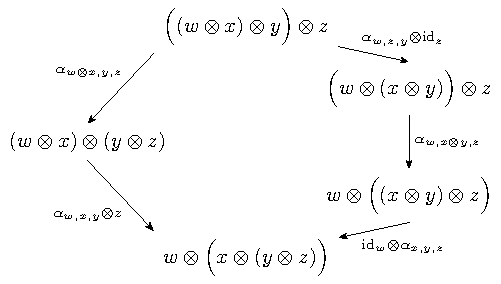
\includegraphics{images/pentagon-equation.pdf} &
    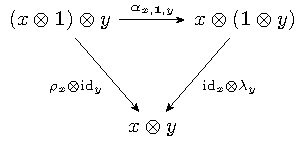
\includegraphics{images/triangle-equation.pdf} \\
    (a) & (b)
  \end{tabular}
  \caption[五边形方程和三角形方程对应的交换图]{五边形方程 (a) 和三角形方程 (b) 对应的交换图。}
  \label{fig:pentagon-triangle-equation}
\end{figure}

如果上述定义中的 $\similarrightarrow$ 可以取为等号,则称该张量范畴是\emph{严格} (strict) 的,此时 $\alpha$、$\lambda$ 和 $\rho$ 均为恒等变换。根据 MacLane \emph{一致性定理} (coherence theorem),每个张量范畴都等价于一个严格张量范畴\cite{maclane2013categories}。因此我们之后可以只考虑严格张量范畴的情况。此时张量积表达式中的括号和单位对象都可以忽略。

一个张量范畴也是一个\emph{幺半群} (monoid),因为范畴的单位对象可以作为群的单位元,而张量积可以作为群乘法。所以张量范畴也被称为\emph{幺半范畴} (monoidal category)。

\subsection{对偶}

类似于对偶空间的概念,我们可以在张量范畴中引入\emph{对偶} (dual) 的概念。$x\in\mathcal{C}$ 的\emph{右对偶} (right dual) $x^\vee$ 通过以下两个态射定义:
\begin{equation}
  e_x\colon x^\vee\otimes x\to\1, \quad i_x\colon\1\to x\otimes x^\vee,
\end{equation}
它们需要满足\emph{刚性公理} (rigidity axioms):
\begin{equation}
  \begin{aligned}
    (\id_x\otimes e_x) \circ (i_x\otimes\id_x) &= \id_x, \\
    (e_x\otimes\id_{x^\vee}) \circ (\id_{x^\vee}\otimes i_x) &= \id_{x^\vee}.
  \end{aligned}
\end{equation}
如果在弦图中省略单位元(对应于物理中的真空态),则 $e_x$ 和 $i_x$ 可以表示为
\begin{equation}
  \tikzinput{dual-1},
  \qquad
  \tikzinput{dual-2}.
\end{equation}
这可以类比于量子力学中的湮灭与产生算符。(右对偶的)刚性公理则可表示为
\begin{equation}
  \tikzinput{rigidity-axioms-1},
  \qquad
  \tikzinput{rigidity-axioms-2}.
  \label{eq:rigidity-axioms-diagrams}
\end{equation}

同理,我们还可以定义\emph{左对偶} (left dual):
\begin{equation}
  e'_x \colon x\otimes \ldual{x}\to\1, \quad i'_x\colon \1\to\ldual{x}\otimes x.
  \label{eq:left-dual}
\end{equation}
这实际上只需要对上面的图沿水平方向做一下镜像操作。如果 $\mathcal{C}$ 中的每个对象既有左对偶也有右对偶,则称其为是\emph{刚性} (rigid) 的或\emph{自治} (autonomous) 的;而如果 $\forall x\in\mathcal{C}$,都有 $x=x^\vee$,则称 $\mathcal{C}$ 是\emph{自对偶} (self-dual) 的。

\subsection{中枢与球状结构}

我们知道有限维向量空间 $V$ 的二重对偶 $V^{\vee\vee}$ 同构于 $V$。这在张量范畴中的推广即为\emph{中枢} (pivotal) 结构,它是由以下的自然同构给出的:
\begin{equation}
  \delta_x \colon x \similarrightarrow x^{\vee\vee}, \quad \forall x\in\mathcal{C},
\end{equation}
且需满足
\begin{equation}
  \delta_{x\otimes y} = \delta_x\otimes\delta_y, \quad
  \delta_{\1} = \id_{\1}, \quad
  \delta_{x^\vee} = (\delta_x^\vee)^{-1}.
\end{equation}
根据右对偶的定义,可有
\begin{equation}
  e_x\colon x^\vee\otimes x \similarrightarrow x^\vee\otimes x^{\vee\vee}\to\1, \quad
  i_x\colon \1\to x\otimes x^\vee \similarrightarrow x^{\vee\vee}\otimes x^\vee.
\end{equation}
对比式~\eqref{eq:left-dual},可以发现 $x^{\vee\vee}$ 也是 $x^\vee$ 的左对偶。若令 $y=x^\vee$,即有 $\ldual{y}=y^\vee$,也就是说在中枢范畴中可以不再区分左右对偶。

对于中枢范畴 $\mathcal{C}$ 中的自同态 $f\in\End_{\mathcal{C}}(x)$,可以定义\emph{左右迹} (left/right trace):
\begin{equation}
  \begin{aligned}
    \tr_{\text{L}} f &\colon \1
      \xrightarrow{i_{x^\vee}} x^\vee\otimes x^{\vee\vee}
      \xrightarrow{\id_{x^\vee}\otimes\delta_x^{-1}} x^\vee\otimes x
      \xrightarrow{\id_{x^\vee}\otimes f} x^\vee\otimes x
      \xrightarrow{e_x} \1, \\
    \tr_{\text{R}} f &\colon \1
      \xrightarrow{i_x} x\otimes x^\vee
      \xrightarrow{f\otimes\id_{x^\vee}} x\otimes x^\vee
      \xrightarrow{\delta_x\otimes\id_{x^\vee}} x^{\vee\vee}\otimes x^\vee
      \xrightarrow{e_{x^\vee}} \1.
  \end{aligned}
\end{equation}
当 $f=\id_x$ 时,还可以定义\emph{左右维数} (left/right dimension):
\begin{equation}
  \dim_{\text{L}} x \coloneq \tr_{\text{L}}\id_x, \quad
  \dim_{\text{R}} x \coloneq \tr_{\text{R}}\id_x.
  \label{eq:left-right-dimension}
\end{equation}
迹和维数可以用下图来描述:
\begin{equation}
  \tr_{\text{L}}  f = \tikzinput{trace-1} \, , \quad
  \tr_{\text{R}}  f = \tikzinput{trace-2} \, ; \quad
  \dim_{\text{L}} x = \tikzinput{dimension-1} \!, \quad
  \dim_{\text{R}} x = \tikzinput{dimension-2} \!.
\end{equation}
如果对于任意的 $f\in\End_{\mathcal{C}}(x)$ 都有 $\tr_{\text{L}}f=\tr_{\text{R}}f$,则称 $\mathcal{C}$ 是\emph{球状} (spherical) 的。

\subsection{融合范畴}

范畴中还可以引入\emph{直和} (direct sum) 的结构。若范畴 $\mathcal{C}$ 中的对象均可分解为\emph{简单对象} (simple object) 的直和:
\begin{equation}
  x = \bigoplus_{i\in I} n_i x_i, \quad \forall x \in \mathcal{C},
\end{equation}
其中 $x_i\in\mathcal{C}$ 是简单对象,$I$ 是由非零简单对象(等价类)构成的指标集,而系数 $n_i\in\mathbb{Z}_+$,则称 $\mathcal{C}$ 是一个\emph{半单范畴} (semi-simple category)。简单对象的例子包括向量空间范畴 $\mathbf{Vec}$ 中的一维空间(直线),以及 Abel 群范畴 $\mathbf{Ab}$ 中的单群。

若张量范畴 $\mathcal{C}$ 同时也是半单的,并且简单对象只有有限多个,那么这样的 $\mathcal{C}$ 称为\emph{融合范畴} (fusion category)\cite{bakalov2001lectures,kitaev2006anyons,bruillard2016rank,aasen2020topological,lou2021dummy}。此时简单对象的张量积可以写成:
\begin{equation}
  x_a \otimes x_b = \bigoplus_c N_{ab}^c x_c,
\end{equation}
其中 $N_{ab}^c\in\mathbb{Z}_+$,称为\emph{融合系数} (fusion coefficient)。在物理学中一般可以假设 $N_{ab}^c$ 只能取到 0 或 1,即是否允许该融合发生。所有允许的融合称为\emph{融合规则} (fusion rule)。融合范畴还要与张量范畴的结构相容,这意味着
\begin{equation}
  N_{\1 a}^b = N_{a\1}^b = \delta_{ab}, \quad
  \sum_x N_{ax}^z N_{bc}^x = \sum_y N_{ab}^y N_{yc}^z.
\end{equation}
我们还要求融合范畴是刚性且自对偶的,此时可以证明
\begin{equation}
  N_{ab}^c = N_{ba}^c = N_{ac}^b = N_{ca}^b = N_{bc}^a = N_{cb}^a,
\end{equation}
即融合系数关于所有指标均对称。

定义矩阵 $(N_a)_{bc}\coloneq N_{ab}^c$,根据 Perron--Frobenius 定理,可知 $N_a$ 存在最大的非负特征值,这定义为简单对象 $a$ 的\emph{量子维数} (quantum dimension)或 Perron--Frobenius 维数 $d_a$。可以证明,量子维数与式~\eqref{eq:left-right-dimension} 中通过迹定义的维数是相同的。融合范畴 $\mathcal{C}$ 的\emph{总量子维数} (total quantum dimension) 定义为
\begin{equation}
  D = \sqrt{\sum_{i\in I} d_i^2}.
\end{equation}

融合的逆运算是\emph{分裂} (splitting)。简单对象的融合与分裂都可以用弦图来表示:
\begin{equation}
  \tikzinput{fusion-tree-1}
  \in \Hom_{\mathcal{C}}(a\otimes b, c) \eqcolon V^{ab}_c, \quad
  \tikzinput{fusion-tree-2}
  \in \Hom_{\mathcal{C}}(c, a\otimes b) \eqcolon V_{ab}^c.
\end{equation}
由于 $\mathcal{C}$ 的刚性和自对偶性,我们可以省略弦图中的箭头。此时,$\Hom_{\mathcal{C}}(a\otimes b,c)$ 和 $\Hom_{\mathcal{C}}(c,a\otimes b)$ 都是向量空间,分别记为 $V^{ab}_c$ 和 $V_{ab}^c$,上面的“融合树”正是对应的基向量。这两个向量空间的维数相等,都等于融合系数 $N_{ab}^c$。

下面我们考虑向量空间 $V^{abc}_d$,它表示从 $a\otimes b\otimes c$ 到 $d$ 的融合。由于 $\mathcal{C}$ 是严格的,$(a\otimes b)\otimes c$ 和 $a\otimes(b\otimes c)$ 的结果相同(都等于 $d$),但却会给出两种融合树的分支结构:
\begin{equation}
  \tikzinput{f-symbol-1}
  \in \bigoplus_x V^{ab}_x \otimes V^{xc}_d \simeq V^{abc}_d, \quad
  \tikzinput{f-symbol-2}
  \in \bigoplus_x V^{ay}_d \otimes V^{bc}_y \simeq V^{abc}_d.
\end{equation}
联系这两组基的变换称为 \emph{$F$ 移动} ($F$ move):
\begin{equation}
  \tikzinput{f-symbol-1}
  = \sum_y \, \bigl[ F^{abc}_d \bigr]_{xy}
  \tikzinput{f-symbol-2}.
  \label{eq:f-move}
\end{equation}
式中的系数 $[F^{abc}_d]_{xy}$ 称为 \emph{$F$ 符号} ($F$ symbol),它一共有 6 个指标。$\mathcal{C}$ 中的 $F$ 符号并不是独立的。如图~\ref{fig:f-symbols-pentagon-equation} 所示,它们所满足的约束条件同样也是五边形方程。

\begin{figure}[htb]
  \centering
  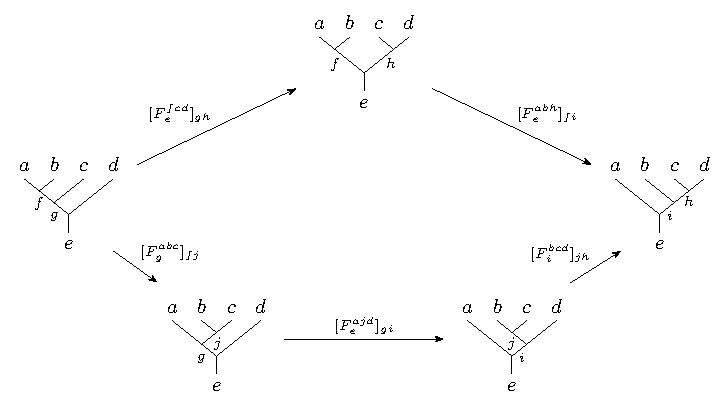
\includegraphics{images/f-symbols-pentagon-equation.pdf}
  \caption[$F$ 符号所满足的五边形方程]{$F$ 符号所满足的五边形方程,对应的融合空间是 $\Hom_{\mathcal{C}}(a\otimes b\otimes c\otimes d,e)$,即 $V^{abcd}_e$。}
  \label{fig:f-symbols-pentagon-equation}
\end{figure}

一个融合范畴可由以下几组数据完全确定:
\begin{itemize}
  \item 简单对象(等价类)的集合 $\{a,b,c,\dots\}$;
  \item 融合系数 $N_{ab}^c$ 或者对应的融合规则;
  \item $F$ 符号 $[F^{abc}_d]_{xy}$。
\end{itemize}
利用这些数据可以对任意弦图进行化简或求值。如果一个弦图没有端点(即“外腿”),那么它的化简结果将是一个复数。根据上文,我们可以进行的操作有:
\begin{itemize}
  \item 任意的连续变形,这是由刚性公理式~\eqref{eq:rigidity-axioms-diagrams} 和自对偶性保证的;
  \item $F$ 移动,即式~\eqref{eq:f-move};
  \item 环路消除,这会得到相应的量子维数:
    \begin{equation}
      \tikzinput{loop-removal-1}
      \! = d_a, \quad
      \tikzinput{loop-removal-2}
      \! = \delta_{ac} \sqrt{\frac{d_b d_{b'}}{d_a}} \enspace
      \tikzinput{loop-removal-3}.
    \end{equation}
\end{itemize}

\subsection{融合范畴的例子}
\label{subsec:fusion-category-examples}

下面我们给出一些融合范畴的例子\cite{rowell2009classification}。这里只列出了非平凡的 $F$ 符号,对于其他合法的融合树,它们之间基变换的 $F$ 符号都等于 1。

\paragraph{Semion}

\begin{itemize}
  \item 简单对象:$\{\1, s\}$;
  \item 量子维数:$d_{\1}=d_s=1$;
  \item 总量子维数:$D=\sqrt2$;
  \item 融合规则:
    \begin{fusionrules}{|c|cc|}
      $\otimes$ & $\1$ & $s$  \\ \hline
      $\1$      & $\1$ & $s$  \\
      $s$       & $s$  & $\1$ \\
    \end{fusionrules}
  \item $F$ 符号:$[F^{sss}_s]_{\1\1}=-1$。
\end{itemize}

\paragraph{Fibonacci}

\begin{itemize}
  \item 简单对象:$\{\1, \tau\}$;
  \item 量子维数:$d_{\1}=1, \, d_\tau=\varphi$;
  \item 总量子维数:$D=\sqrt{\frac{5+\sqrt5}{2}}=2\cos\frac{\pi}{10}$;
  \item 融合规则:
    \begin{fusionrules}{|c|cc|}
      $\otimes$ & $\1$   & $\tau$ \\ \hline
      $\1$      & $\1$   & $\tau$ \\
      $\tau$    & $\tau$ & $\1\oplus\tau$ \\
    \end{fusionrules}
  \item $F$ 符号:
    $
      [F^{\tau\tau\tau}_\tau]_{ij} = \dfrac1\varphi \begin{pmatrix} 1 & \sqrt\varphi \\ \sqrt\varphi & -1 \end{pmatrix}, \,
      i,j \in \{\1, \tau\}
    $。
\end{itemize}

这里的 $\varphi=(1+\sqrt5)/2$ 是黄金比。

\paragraph{Ising}

\begin{itemize}
  \item 简单对象:$\{\1, \sigma, \psi\}$;
  \item 量子维数:$d_{\1}=d_\psi=1, \, d_\sigma=\sqrt2$;
  \item 总量子维数:$D=2$;
  \item 融合规则:
    \begin{fusionrules}{|c|ccc|}
      $\otimes$ & $\1$     & $\sigma$       & $\psi$   \\ \hline
      $\1$      & $\1$     & $\sigma$       & $\psi$   \\
      $\sigma$  & $\sigma$ & $\1\oplus\psi$ & $\sigma$ \\
      $\psi$    & $\psi$   & $\sigma$       & $\1$     \\
    \end{fusionrules}
  \item $F$ 符号:
    $
      [F^{\psi\sigma\psi}_\sigma]_{\sigma\sigma} = [F^{\sigma\psi\sigma}_\psi]_{\sigma\sigma} = -1, \,
      [F^{\sigma\sigma\sigma}_\sigma]_{ij} = -\dfrac{1}{\sqrt2} \begin{pmatrix} 1 & 1 \\ 1 & -1 \end{pmatrix}, \,
      i,j \in \{\1, \psi\}
    $。
\end{itemize}

\paragraph{Toric code}

\begin{itemize}
  \item 简单对象:$\{\1, e, m, f\}$;
  \item 量子维数:$d_{\1}=d_e=d_m=d_f=1$;
  \item 总量子维数:$D=2$;
  \item 融合规则:
    \begin{fusionrules}{|c|cccc|}
      $\otimes$ & $\1$ & $e$  & $m$  & $f$  \\ \hline
      $\1$      & $\1$ & $e$  & $m$  & $f$  \\
      $e$       & $e$  & $\1$ & $f$  & $m$  \\
      $m$       & $m$  & $f$  & $\1$ & $e$  \\
      $f$       & $f$  & $m$  & $e$  & $\1$ \\
    \end{fusionrules}
  \item $F$ 符号:都等于 1。
\end{itemize}

\subsection{更复杂的例子:\texorpdfstring{$\mathcal{A}_{k+1}$}{𝒜ₖ₊₁} 范畴}
\label{subsec:A-k+1-category}

$\mathcal{A}_{k+1}$ 范畴\cite{coquereaux2007racah,aasen2020topological,chen2022galois}也称 $\mathfrak{su}(2)_k$ 模型,它最初来自于对 Lie 代数表示的研究。该范畴中共有 $k+1$ 个简单对象,标记为 $0,\frac12,1,\dots,\frac k2$,对应的量子维数为
\begin{equation}
  d_i = \frac{\sin\frac{(2i+1)\pi}{k+2}}{\sin\frac{\pi}{k+2}}, \quad i = 0,1,2,\dots,k.
\end{equation}
计算可得总量子维数
\begin{equation}
  D = \frac12 \left( \cot^2 \frac{\pi}{2k+4} - 1 \right).
\end{equation}
融合规则由下式确定:
\begin{equation}
  N_{ab}^c = \begin{cases}
    1, & a+b\geqslant c, \, b+c\geqslant a, \, c+a\geqslant b, \, a+b+c\leqslant k, \, a+b+c\in\mathbb{Z}; \\
    0, & \text{otherwise}.
  \end{cases}
\end{equation}
例如当 $k=1$ 和 2 时,融合规则分别为
\begin{fusionrules}{|c|cc|}
  $\otimes$ & 0 & ½ \\ \hline
  0         & 0 & ½ \\
  ½         & ½ & 0 \\
\end{fusionrules}
和
\begin{fusionrules}{|c|ccc|}
  $\otimes$ & 0 & ½          & 1 \\ \hline
  0         & 0 & ½          & 1 \\
  ½         & ½ & $0\oplus1$ & ½ \\
  1         & 1 & ½          & 0 \\
\end{fusionrules}。

\begin{equation}
  G^{abc}_{def} = \begin{Bmatrix} a & b & c \\ d & e & f \end{Bmatrix}_q (-1)^p,
\end{equation}
式中
\begin{equation}
  p = \frac{3(a+b+c+d+e+f)^2 - (a+d)^2 - (b+e)^2 - (c+f)^2}{2},
\end{equation}
而 $\{\dots\}_q$ 称为 \emph{$q$-变形 Wigner $6j$ 符号} ($q$-deformed Wigner $6j$ symbol),其定义为
\begin{align}
  \begin{Bmatrix} j_1 & j_2 & j_3 \\ j_4 & j_5 & j_6 \end{Bmatrix}_q
  &= \Delta(j_1,j_2,j_3) \, \Delta(j_1,j_5,j_6) \, \Delta(j_4,j_2,j_6) \, \Delta(j_4,j_5,j_3) \notag \\
  &\times \sum_{z=m}^M \frac{(-1)^z [z+1]!}{[z-a_1]![z-a_2]![z-a_3]! [b_1-z]![b_2-z]![b_3-z]!},
\end{align}
其中
\begin{align}
  q    &= \exp\frac{2\pi\ii}{k+2}, \\
  [n]  &= \frac{q^{m/2} - q^{-m/2}}{q^{1/2} - q^{-1/2}} = \frac{\sin\frac{n\pi}{k+2}}{\sin\frac{\pi}{k+2}}, \\
  [n]! &= \begin{cases}
    \prod_{i=1}^{n} [n], & n \geqslant 1; \\
    1                    & n = 0,
  \end{cases} \\
  \Delta(x,y,z) &= \sqrt{\frac{[x+y-z]! [y+z-x]! [z+x-y]!}{[x+y+z+1]!}},
\end{align}
此外 $a_1=j_1+j_2+j_3$,$a_2=j_1+j_5+j_6$,$a_3=j_2+j_4+j_6$,$a_4=j_3+j_4+j_5$,$b_1=j_1+j_2+j_4+j_5$,$b_2=j_2+j_3+j_5+j_6$,$b_3=j_1+j_3+j_4+j_6$,而对 $z$ 的求和为从 $m=\max\{a_1,a_2,a_3,a_4\}$ 到 $M=\min\{b_1,b_2,b_3\}$ 的整数。

\subsection{模张量范畴与共形场论}

在二维共形场论 (conformal field theory, CFT) 的最小模型 (minimal model) 中,初级场 (primary field) 之间也存在融合规则\cite{ginsparg1988applied,francesco2012conformal}:
\begin{equation}
  \phi_{(r,s)} \times \phi_{(m,n)}
  = \sum_{\substack{k=1+|r-m| \\ k+r+m=1 \bmod 2}}^{k_{\max}} \,
    \sum_{\substack{l=1+|s-n| \\ l+s+n=1 \bmod 2}}^{l_{\max}} \phi_{(k,l)},
\end{equation}
式中
\begin{equation}
  \begin{aligned}
    k_{\max} &= \min(r+m-1, 2p'-1-r-m), \\
    l_{\max} &= \min(s+n-1, 2p-1-s-n),
  \end{aligned}
\end{equation}
而 $p$ 和 $p'$ 是两个互素的整数,它们确定了最小模型 $\mathcal{M}(p,p')$。以二维临界 Ising 模型为例,它是最小模型 $\mathcal{M}(4,3)$,其中的初级场除了恒等算符 $\1$ 之外,还包括自旋 $\sigma$ 和能量密度 $\epsilon$。它们满足的融合规则为:
\begin{equation}
  \sigma\times\sigma = \1+\epsilon, \quad
  \sigma\times\epsilon = \sigma, \quad
  \epsilon\times\epsilon = \1.
\end{equation}
这与上面 Ising 融合范畴中(非平凡)的融合规则是完全一致的。

事实上,我们在 \ref{subsec:fusion-category-examples} 和 \ref{subsec:A-k+1-category} 小节中给出的这几个例子不仅是融合范畴,还是所谓\emph{模张量范畴} (modular tensor category, MTC)\cite{bakalov2001lectures,kitaev2006anyons,bruillard2016rank,beer2018categories,kong2022invitation}。它在融合范畴的基础上加入了\emph{编织} (braiding)、\emph{丝带} (ribbon) 的结构以及\emph{非简并} (non-degeneracy) 的条件,其中定义了\emph{扭转} (twist):
\begin{equation}
  \theta_x = \tikzinput{twist} \, , \quad x \in \mathcal{C},
\end{equation}
\emph{$S$ 矩阵} ($S$ matrix):
\begin{equation}
  S_{ij} = \frac1D \, \tikzinput{s-matrix}, \quad i,j \in I,
\end{equation}
\emph{Gauss 和} (Gauss sums):
\begin{equation}
  p^{\pm} = \sum_{i\in I} \theta_i^{\pm1} d_{i}^2.
\end{equation}
Gauss 和与 $\mathcal{C}$ 的总量子维数相关:
\begin{equation}
  p^+ p^- = D^2,
\end{equation}
而其比值定义为
\begin{equation}
  \zeta = \left( \frac{p^+}{p^-} \right)^{1/6}.
\end{equation}
可以证明模张量范畴中融合系数与 $S$ 矩阵之间存在如下关系\cite{verlinde1988fusion,bakalov2001lectures,huang2005vertex,bruillard2016rank}:
\begin{equation}
  N_{ij}^k = \sum_r \frac{S_{ir} S_{jr} S_{k^\vee r}}{S_{\1 r}},
\end{equation}
这被称为 \emph{Verlinde 公式} (Verlinde formula)。此外,还存在 \emph{Vafa 定理} (Vafa's theorem),即 $\theta_i$ 和 $\zeta$ 都是单位根\cite{bakalov2001lectures}。此时令
\begin{equation}
  \theta_i = \ee^{2\pi\ii\Delta_i}, \quad
  \zeta = \ee^{2\pi\ii c/24},
\end{equation}
% TODO: $\Delta_i$ conformal or scaling dimension?
可知式中 $\Delta_i$ 和 $c$ 都是有理数。它们正是\emph{有理共形场论} (rational CFT, RCFT) 中的\emph{共形维数} (conformal dimension) 和\emph{中心荷} (central charge)。

\section{拓扑序与弦网模型}

\subsection{拓扑序}

在 Landau 相变理论中,不同的相可根据对称性来确定,并可通过\emph{序参量} (order parameter) 来刻画。相变则通过对称性破缺来描述。但在 20 世纪 80 年代以来,随着分数量子 Hall 效应、高温超导等现象的发现,人们意识到 Landau 的对称性破缺理论并不足以描述所有的物态。\emph{拓扑序} (topological order) 的提出即为了描述这些物态的性质,并对其进行分类。

在 2+1D 中,拓扑序可由下面两条性质来确定\cite{zeng2019introduction}:
\begin{itemize}
  \item 基态的拓扑简并;
  \item 非 Abel 的几何相。
\end{itemize}

\subsection{Toric code 模型}

拓扑序的一个基本且重要的例子是 Toric code 模型\cite{kitaev2003fault}。它定义在一个二维正方形网格 (square lattice) 上,每条边上都存在一个自旋 $1/2$ 的自由度 $\sigma_i$。一般我们选取周期性边界条件,即环面拓扑。其 Hamilton 量定义为
\begin{equation}
  H = -\sum_{\bm{v}} A_{\bm{v}} - \sum_{\bm{p}} B_{\bm{p}}, \quad
  A_{\bm{v}} = \prod_{i\in\operatorname{star}(\bm{v})} \sigma_i^x, \quad
  B_{\bm{p}} = \prod_{i\in\operatorname{boundary}(\bm{p})} \sigma_i^z,
  \label{eq:toric-code-hamiltonian}
\end{equation}
其中 $\sum_{\bm{v}}$ 和 $\sum_{\bm{p}}$ 分别表示对所有的顶点 (vertex) 和方块\footnote{在其他网格中也可以是其他形状。} (plaquette) 求和,如图~\ref{fig:toric-code-vertex-plaquette} 所示。

\begin{figure}[htb]
  % TODO: update image
  \centering
  \includegraphics[width=0.5\textwidth]{images/temp/ToricCodeLattice.png}
  \caption[Toric code 中的顶点和方块]{正方形网格上 Toric code 中的顶点 ($\bm{v}$) 和方块 ($\bm{p}$),它们各包含 4 个自旋自由度。}
  \label{fig:toric-code-vertex-plaquette}
\end{figure}

Toric code 中存在 $e$ 和 $m$ 两种激发态,分别由 $\sigma^z$ 和 $\sigma^x$ 组成的弦算符产生。$e$ 和 $m$ 分别绕对方一圈(e.g. $e$ 闭弦 + $m$ 开弦),会给出 -1 的相位。

Toric code 存在 4 种任意子:$\1$、$e$、$m$、$f=e\times m$。它们的 fusion rules 如下……

基态简并度与空间底流形的拓扑有关:$d=2^{2^g}=4^g$,其中 $g$ 为空间的\emph{亏格} (genus)。

\subsection{弦网模型}

\emph{弦网模型} (string-net model)\cite{levin2005string,levin2006detecting} 可以视为 Toric code 模型的一种推广,它是通过 \ref{sec:tensor-category-fusion-category} 节介绍的张量融合范畴来定义的\footnote{准确来说要求模张量范畴。}。弦网模型一般定义在一个三分支 (trivalent) 的网格上,网格的边上带有“弦”的自由度。对于一个具体的弦网模型,我们需要给出下列几组数据:
\begin{itemize}
  \item \emph{弦的类型},按照量子力学的语言也被称为\emph{超选择分区} (superselection sector),它相当于融合范畴中简单对象的集合;
  \item \emph{弦的取向},相当于指定了简单对象的对偶;
  \item \emph{分支规则},相当于融合规则,规定了哪些弦允许汇聚于一点。
\end{itemize}

根据张量融合范畴的精神,弦网模型的基态波函数 $\Phi$ 应该满足下面的约束条件:
\begin{equation}
  % TODO: update image and conventions
  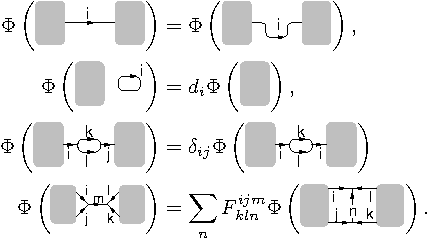
\includegraphics{images/temp/string-net-wave-function.pdf}
\end{equation}
这里的 $F^{ijm}_{kln}$ 是 $F$ 符号的另一种记法,它与 $F[...]$ 的关系将在 [...] 中给出。

在六边形网格 (hexagonal lattice) 上定义的弦网模型,其 Hamilton 量由下式给出:
\begin{equation}
  H = -\sum_{\bm{v}} A_{\bm{v}} - \sum_{\bm{p}} B_{\bm{p}}.
  \label{eq:string-net-hamiltonian}
\end{equation}
与式~\eqref{eq:toric-code-hamiltonian} 类似,这里 $\bm{v}$ 和 $\bm{p}$ 也表示顶点和方块。$A_{\bm{v}}$ 称为\emph{电荷算符} (electric charge operator):
\begin{equation}
  % A_{\bm{v}} \ket{...} = \delta_{ijk} \ket{...}
  \includegraphics{images/temp/string-net-electric-charge.pdf}
\end{equation}
$B_{\bm{p}}$ 称为\emph{磁通量算符} (magnetic flux operator):
\begin{equation}
  B_{\bm{p}} = \sum_{s=0}^N \frac{d_s}{D} B_{\bm{p}}^s,
\end{equation}
其中
\begin{equation}
  \begin{gathered}
    % B_{\bm{p}}^s \ket{...} = \sum ... \ket{...}
    \includegraphics{images/temp/string-net-magnetic-flux.pdf}, \\
    B_{\bm{p},ghijkl}^{s,g'h'i'j'k'l'}(abcdef) =
      F^{al^*g}_{s^*g'l'^*}
      F^{bg^*h}_{s^*h'g'^*}
      F^{ch^*i}_{s^*i'h'^*}
      F^{di^*j}_{s^*j'i'^*}
      F^{ej^*k}_{s^*k'j'^*}
      F^{fk^*l}_{s^*l'k'^*}.
  \end{gathered}
\end{equation}
可以验证 $A_{\bm{v}}$ 与 $B_{\bm{p}}$ 是对易的,因而 Hamilton 量式~\eqref{eq:string-net-hamiltonian} 严格可解。
